\section{Использование прогнозного управления}

\subsection*{Алгоритм прогнозного управления}

Прогнозное управление (Model Predictive Control, MPC) представляет собой один из наиболее
перспективных подходов к управлению нелинейными системами с ограничениями. В отличие от
традиционных методов управления, таких как ПИД-регулирование или управление в
скользящих режимах, прогнозное управление основано на решении задачи оптимизации
на каждом шаге управления с использованием математической модели объекта для прогнозирования его будущего поведения.

\paragraph*{Математическая формулировка прогнозного управления для пневмопривода.}

Принцип работы прогнозного управления заключается в использовании модели объекта для
прогнозирования его будущего поведения на определенном горизонте прогноза $N_p$ и определении
последовательности управляющих воздействий $\{u(k), u(k+1), ..., u(k+N_c-1)\}$ на горизонте управления
$N_c$ ($N_c \leq N_p$), минимизирующей заданную целевую функцию.
\nomenclature{$N_p$}{Горизонт прогноза\nomrefeqpage}
\nomenclature{$N_c$}{Горизонт управления\nomrefeqpage}

Для пневматического привода с дискретными распределителями задача прогнозного управления
формулируется следующим образом. В каждый момент времени $k$ известно текущее
состояние системы $x(k)$, включающее положение штока, скорость его движения и давления
в рабочих полостях. С использованием математической модели пневмопривода
выполняется прогноз состояний системы $\{x(k+1|k), x(k+2|k), ..., x(k+N_p|k)\}$ на
горизонте прогноза $N_p$ для различных последовательностей управляющих воздействий. На
основе полученных прогнозов выбирается такая последовательность управляющих
воздействий $\{u(k|k), u(k+1|k), ..., u(k+N_c-1|k)\}$, которая минимизирует целевую
функцию, учитывающую ошибку позиционирования, быстродействие системы и число переключений
распределителей. После чего применяется первое управляющее воздействие из
оптимальной последовательности $u(k) = u(k|k)$. На следующем шаге
управления $(k+1)$ процедура повторяется с учетом нового измеренного состояния системы $x(k+1)$.

Математическая модель электропневматического привода с дискретными распределителями в
упрощенном представлении описывается следующей системой дифференциальных уравнений:

\begin{equation}
	\begin{cases}
		\dot{x} = v;                                                                                                  \\
		\dot{v} = \frac{1}{M}(p_1 F_1 - p_2 F_2 - R_{\text{тр}}(v));                                                  \\
		\dot{p}_1 = \frac{\gamma R T}{V_1(x)}(\dot{m}_{\text{вх},1} - \dot{m}_{\text{вых},1} - \frac{p_1}{R T}F_1 v); \\
		\dot{p}_2 = \frac{\gamma R T}{V_2(x)}(\dot{m}_{\text{вх},2} - \dot{m}_{\text{вых},2} + \frac{p_2}{R T}F_2 v), \\
	\end{cases}
\end{equation}
где $x$ -- положение штока;
$v$ -- скорость штока;
$p_1$ и $p_2$ -- давления в поршневой и штоковой полостях соответственно;
$M$ -- масса подвижных частей;
$F_1$ и $F_2$ -- эффективные площади поршня
$R_{\text{тр}}(v)$ -- сила трения;
$\gamma$ -- показатель адиабаты;
$R$ -- газовая постоянная;
$T$ -- температура;
$V_1(x)$ и $V_2(x)$ -- объемы полостей;
$\dot{m}_{\text{вх},i}$ и $\dot{m}_{\text{вых},i}$ -- массовые расходы воздуха
через впускные и выпускные распределители для $i$-й полости.

Массовые расходы воздуха через распределители зависят от
их управляющих сигналов $u_i \in \{0, 1\}$ и могут быть описаны следующими выражениями:

\begin{equation}
	\begin{aligned}
		\dot{m}_{\text{вх},1}  & = u_1 \cdot C_1 \cdot f(p_\text{п}, p_1);    \\
		\dot{m}_{\text{вых},1} & = u_2 \cdot C_2 \cdot f(p_1, p_\text{атм});  \\
		\dot{m}_{\text{вх},2}  & = u_3 \cdot C_3 \cdot f(p_\text{п}, p_2);    \\
		\dot{m}_{\text{вых},2} & = u_4 \cdot C_4 \cdot f(p_2, p_\text{атм}) , \\
	\end{aligned}
\end{equation}
где $C_i$ -- проводимость $i$-го распределителя;
$p_\text{п}$ -- давление питания;
$p_\text{атм}$ -- атмосферное давление;
$f(p_u, p_d)$ -- функция, описывающая расход через распределитель
в зависимости от отношения давлений на входе $p_u$ и выходе $p_d$.

Для докритического режима течения ($p_d/p_u > b_{\text{кр}}$) аппроксимированная функция расхода имеет вид:

\begin{equation}
	f(p_u, p_d) = C_d F_\text{пр} \psi(r) p_u \sqrt{\frac{2}{RT}},
\end{equation}
где $r = p_d/p_u$ -- отношение давлений;
а $\psi(r)$ -- расходная функция, аппроксимированная полиномом:

\begin{equation}
	\psi(r) = 1 - a_1(1-r) - a_2(1-r)^2 - a_3(1-r)^3.
\end{equation}

Для критического режима ($p_d/p_u \leq b_{\text{кр}}$):

\begin{equation}
	f(p_u, p_d) = C_d F_\text{пр} \psi(b_{\text{кр}}) p_u \sqrt{\frac{2}{RT}},
\end{equation}
где $b_{\text{кр}} \approx \num{0.528}$ -- критическое отношение давлений для воздуха;

Особенностью прогнозного управления применительно к пневмоприводу с дискретными
распределителями является дискретный характер управляющих воздействий. В каждый момент времени
распределитель может находиться только в одном из двух состояний: открыт (1) или закрыт (0), что
существенно ограничивает пространство поиска оптимальных управляющих воздействий.
В то же время, за счет комбинации состояний четырех распределителей можно реализовать различные режимы работы привода.

В данной реализации используется 5-режимное управление, где каждый режим
соответствует определенной комбинации состояний распределителей:

\begin{enumerate}[label=\arabic*)]
	\item режим сильного положительного ускорения: $u = [1, 0, 0, 1]$;
	\item режим умеренного положительного ускорения: $u = [1, 0, 0, 0]$;
	\item режим удержания: $u = [0, 0, 0, 0]$;
	\item режим умеренного отрицательного ускорения: $u = [0, 0, 1, 0]$;
	\item режим сильного отрицательного ускорения: $u = [0, 1, 1, 0]$;
\end{enumerate}

\paragraph*{Целевая функция и алгоритм оптимизации.}

Для оценки качества управления используется целевая функция, минимизируемая на горизонте прогноза:

\begin{equation}
	\begin{aligned}
		J & = \sum_{i=1}^{N_p} Q_{\text{поз}} \cdot (x(k+i|k) - x_{\text{зад}})^2 +                 \\
		  & + \sum_{i=1}^{N_p} Q_{\text{скор}} \cdot v(k+i|k)^2 +                                   \\
		  & + \sum_{i=0}^{N_c-1} R_{\text{перекл}} \cdot \sum_{j=1}^{4} |u_j(k+i|k) - u_j(k+i-1|k)|,
	\end{aligned}
\end{equation}
где $Q_{\text{поз}}$ -- весовой коэффициент ошибки позиционирования;
$Q_{\text{скор}}$ -- весовой коэффициент скорости;
$R_{\text{перекл}}$ -- весовой коэффициент переключений распределителей;
$x_{\text{зад}}$ -- заданное положение.
\nomenclature{$Q_{\text{поз}}$}{Весовой коэффициент ошибки позиционирования\nomrefeqpage}
\nomenclature{$Q_{\text{скор}}$}{Весовой коэффициент скорости\nomrefeqpage}
\nomenclature{$R_{\text{перекл}}$}{Весовой коэффициент переключений распределителей\nomrefeqpage}

Первое слагаемое целевой функции отвечает за точность позиционирования,
второе -- за демпфирование колебаний (стремление к нулевой скорости в конце движения), третье -- за минимизацию числа переключений,
что способствует увеличению ресурса распределителей.

Классическая задача прогнозного управления требует решения на каждом шаге задачи оптимизации для
нахождения оптимальной последовательности управляющих воздействий. В случае дискретных распределителей
это задача комбинаторной оптимизации, полный перебор для которой требует значительных
вычислительных затрат. Для $N_c$ шагов управления и 5 возможных
режимов общее число вариантов составляет $5^{N_c}$, что становится
неприемлемым при увеличении горизонта управления.

Для сокращения вычислительной сложности в данной работе предложено использовать эвристический
подход, основанный на адаптивном формировании пространства поиска.
На основе текущего состояния системы (положения, скорости и ошибки позиционирования)
формируется ограниченное подмножество перспективных режимов управления для
первых нескольких шагов. Вместо полного перебора всех возможных последовательностей
длиной $N_c$ строится дерево решений с ограниченным фактором ветвления на каждом уровне. В
зависимости от величины и знака ошибки позиционирования, а также
текущей скорости, определяются предпочтительные режимы управления.
Например, при большой положительной ошибке $(e > \varepsilon_2)$ предпочтительны
режимы сильного и умеренного положительного ускорения; при малой ошибке
$(|e| \leq \varepsilon_1)$ предпочтителен режим удержания; при высокой скорости движения в
сторону, противоположную направлению к целевой точке, предпочтительны режимы торможения.

Алгоритм эвристического поиска оптимальной последовательности управляющих воздействий
может быть представлен следующим образом. На основе текущего состояния
системы $(x, v, p_1, p_2)$ и заданной точности позиционирования определяются
предпочтительные режимы управления для первого шага. Для каждого предпочтительного
режима первого шага прогнозируется состояние системы через один шаг по времени. На основе
прогнозируемого состояния определяются предпочтительные режимы для второго шага
и так далее до достижения заданной глубины поиска или горизонта управления.
Для каждой сформированной последовательности режимов прогнозируется траектория системы на
всем горизонте прогноза и вычисляется значение целевой функции. Затем выбирается
последовательность с минимальным значением целевой функции, и первый
режим из этой последовательности применяется в текущий момент времени.

Процесс генерации последовательностей управляющих воздействий можно описать
с использованием рекурсивного алгоритма. На каждом шаге алгоритм
принимает текущее состояние системы, текущую глубину рекурсии,
частичную последовательность режимов управления и список всех сгенерированных последовательностей.

Алгоритм продолжает работу до тех пор, пока не будет достигнута
максимальная глубина поиска. После этого сформированная последовательность
добавляется в общий список всех последовательностей. Такой подход позволяет
эффективно формировать множество возможных вариантов управления для
последующего анализа и выбора оптимального.

\paragraph*{Реализация алгоритма прогнозного управления.}

Для эффективной реализации алгоритма прогнозного управления пневмоприводом с дискретными
распределителями требуется
решить ряд практических задач. Полная термодинамическая модель пневмопривода слишком сложна
для использования в реальном времени, поэтому при работе алгоритма используется упрощенная модель,
обеспечивающая достаточную точность прогноза при значительно меньших вычислительных затратах.

Горизонт прогноза должен быть достаточно большим для адекватной оценки динамики системы,
но при этом не требовать чрезмерных вычислительных ресурсов. На основе экспериментальных исследований
установлено, что оптимальные значения горизонта прогноза находятся в диапазоне $8 \leq N_p \leq 15$.

Коэффициенты $Q_{\text{поз}}$, $Q_{\text{скор}}$ и $R_{\text{перекл}}$ определяют приоритеты
различных составляющих целевой функции и существенно влияют на поведение системы. Их подбор
осуществляется на основе анализа важности показателей качества.

Для работы в режиме реального времени необходимо оптимизировать алгоритм по быстродействию.
В данной работе это достигается за счет ограничения числа рассматриваемых последовательностей
управляющих воздействий, использования эвристик для отбора перспективных режимов,
адаптивного изменения шага моделирования в зависимости от динамики системы.

Для повышения устойчивости алгоритма к возмущениям и ошибкам модели реализованы защита
от численной нестабильности при моделировании, механизмы безопасного возврата к базовым
режимам управления при невозможности выполнения оптимизации и адаптация параметров в зависимости от текущей ошибки позиционирования.

На рисунке \ref{fig:mpc_transient} показан рассчитанный переходный процесс
пневмопривода с дискретными распределителями при использовании алгоритма прогнозного управления.

\begin{figure}[ht]
	\centering
	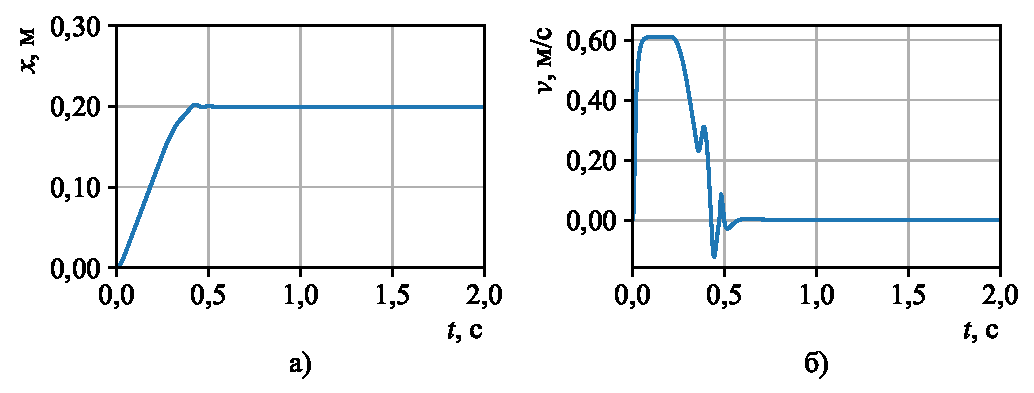
\includegraphics{part3/pneumatic_cylinder_mpc.pdf}
	\caption{Переходный процесс пневмопривода с дискретными распределителями при использовании алгоритма прогнозного управления}
	\label{fig:mpc_transient}
\end{figure}

Система прогнозного управления реализована как иерархическая структура,
включающая верхний уровень (формирование целевой траектории и параметров оптимизации),
средний уровень (решение задачи оптимизации и формирование последовательности управляющих режимов) и
нижний уровень (преобразование режимов в сигналы управления распределителями и их реализация).

Функционирование системы прогнозного управления может быть представлено
в виде блок-схемы, показанной на рисунке~\ref{fig:mpc_block_diagram}.

\begin{figure}[h]
	\centering
	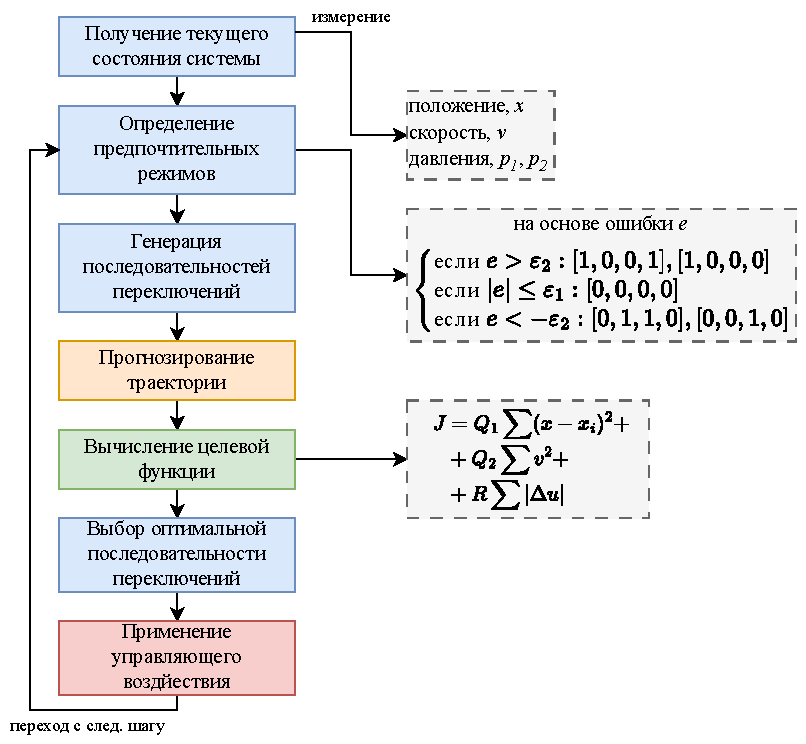
\includegraphics[width=\textwidth]{part3/mpc-block-diagram.pdf}
	\caption{Блок-схема системы прогнозного управления}
	\label{fig:mpc_block_diagram}
\end{figure}

